

\tikzset{every picture/.style={line width=0.75pt}} %set default line width to 0.75pt        

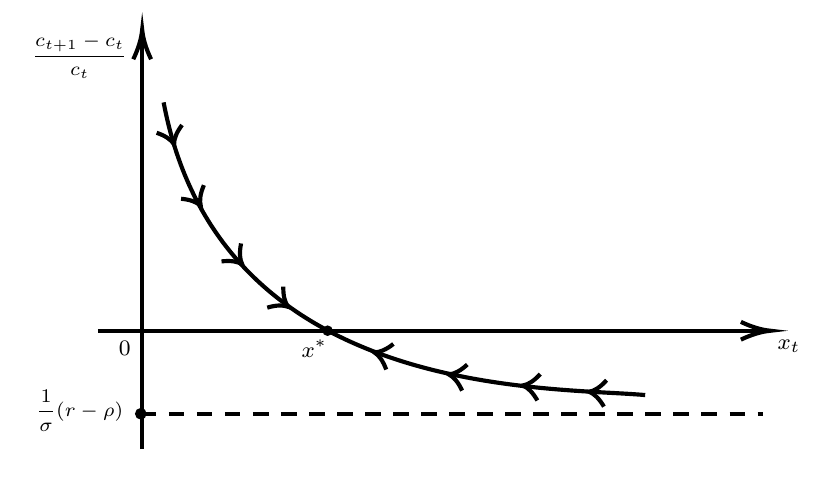
\begin{tikzpicture}[x=0.75pt,y=0.75pt,yscale=-1,xscale=1]
%uncomment if require: \path (0,326); %set diagram left start at 0, and has height of 326

%Straight Lines [id:da7827750633980162] 
\draw [line width=1.5]    (117.33,230) -- (438.33,230) ;
\draw [shift={(441.33,230)}, rotate = 180] [color={rgb, 255:red, 0; green, 0; blue, 0 }  ][line width=1.5]    (14.21,-4.28) .. controls (9.04,-1.82) and (4.3,-0.39) .. (0,0) .. controls (4.3,0.39) and (9.04,1.82) .. (14.21,4.28)   ;
%Straight Lines [id:da48732250900542073] 
\draw [line width=1.5]    (138.67,287.07) -- (138.67,87.98) ;
\draw [shift={(138.67,84.98)}, rotate = 90] [color={rgb, 255:red, 0; green, 0; blue, 0 }  ][line width=1.5]    (14.21,-4.28) .. controls (9.04,-1.82) and (4.3,-0.39) .. (0,0) .. controls (4.3,0.39) and (9.04,1.82) .. (14.21,4.28)   ;
%Straight Lines [id:da22663802590695048] 
\draw [color={rgb, 255:red, 0; green, 0; blue, 0 }  ,draw opacity=1 ][line width=1.5]  [dash pattern={on 5.63pt off 4.5pt}]  (138,270) -- (438,270) ;
\draw [shift={(138,270)}, rotate = 0] [color={rgb, 255:red, 0; green, 0; blue, 0 }  ,draw opacity=1 ][fill={rgb, 255:red, 0; green, 0; blue, 0 }  ,fill opacity=1 ][line width=1.5]      (0, 0) circle [x radius= 1.74, y radius= 1.74]   ;
%Curve Lines [id:da884700851860968] 
\draw [color={rgb, 255:red, 0; green, 0; blue, 0 }  ,draw opacity=1 ][line width=1.5]    (149,119.98) .. controls (176,262.98) and (333.33,256.83) .. (381,260.98) ;
\draw  [color={rgb, 255:red, 0; green, 0; blue, 0 }  ,draw opacity=1 ][line width=1.5]  (157.87,130.87) .. controls (155.23,134.39) and (153.96,137.51) .. (154.04,140.19) .. controls (152.6,137.92) and (149.8,136.06) .. (145.64,134.62) ;
\draw  [color={rgb, 255:red, 0; green, 0; blue, 0 }  ,draw opacity=1 ][line width=1.5]  (186.3,187.94) .. controls (185.45,192.25) and (185.64,195.61) .. (186.87,198) .. controls (184.59,196.57) and (181.26,196.09) .. (176.89,196.59) ;
\draw  [color={rgb, 255:red, 0; green, 0; blue, 0 }  ,draw opacity=1 ][line width=1.5]  (168.39,159.85) .. controls (166.67,163.9) and (166.17,167.22) .. (166.89,169.81) .. controls (164.95,167.95) and (161.79,166.81) .. (157.41,166.4) ;
\draw  [color={rgb, 255:red, 0; green, 0; blue, 0 }  ,draw opacity=1 ][line width=1.5]  (206.66,208.69) .. controls (206.58,213.08) and (207.37,216.35) .. (209,218.49) .. controls (206.51,217.48) and (203.15,217.61) .. (198.93,218.87) ;
\draw  [color={rgb, 255:red, 0; green, 0; blue, 0 }  ,draw opacity=1 ][line width=1.5]  (329.07,263.58) .. controls (326.88,259.77) and (324.53,257.37) .. (322.03,256.38) .. controls (324.68,255.95) and (327.5,254.12) .. (330.46,250.87) ;
\draw  [color={rgb, 255:red, 0; green, 0; blue, 0 }  ,draw opacity=1 ][line width=1.5]  (256.24,248.68) .. controls (254.71,244.55) and (252.79,241.8) .. (250.48,240.41) .. controls (253.17,240.43) and (256.25,239.08) .. (259.71,236.37) ;
\draw  [color={rgb, 255:red, 0; green, 0; blue, 0 }  ,draw opacity=1 ][line width=1.5]  (361.14,266.55) .. controls (358.91,262.76) and (356.53,260.38) .. (354.02,259.42) .. controls (356.67,258.97) and (359.47,257.1) .. (362.4,253.83) ;
\draw  [color={rgb, 255:red, 0; green, 0; blue, 0 }  ,draw opacity=1 ][line width=1.5]  (292.8,258.83) .. controls (290.95,254.84) and (288.82,252.24) .. (286.41,251.04) .. controls (289.1,250.85) and (292.06,249.27) .. (295.3,246.29) ;
%Straight Lines [id:da3437258048528058] 
\draw    (228,229.98) ;
\draw [shift={(228,229.98)}, rotate = 0] [color={rgb, 255:red, 0; green, 0; blue, 0 }  ][fill={rgb, 255:red, 0; green, 0; blue, 0 }  ][line width=0.75]      (0, 0) circle [x radius= 2.01, y radius= 2.01]   ;

% Text Node
\draw (84,86) node [anchor=north west][inner sep=0.75pt]  [font=\scriptsize] [align=left] {$\displaystyle \frac{c_{t+1} -c_{t}}{c_{t}}$};
% Text Node
\draw (214,233) node [anchor=north west][inner sep=0.75pt]  [font=\footnotesize] [align=left] {$\displaystyle x^{*}$};
% Text Node
\draw (443.33,233) node [anchor=north west][inner sep=0.75pt]  [font=\footnotesize] [align=left] {$\displaystyle x_{t}$};
% Text Node
\draw (126,233.66) node [anchor=north west][inner sep=0.75pt]  [font=\footnotesize] [align=left] {$\displaystyle 0$};
% Text Node
\draw (86,257) node [anchor=north west][inner sep=0.75pt]  [font=\scriptsize] [align=left] {$\displaystyle \frac{1}{\sigma }( r-\rho )$};


\end{tikzpicture}